% Main manuscript, following the PNAS LaTeX template (pnas-new.cls, research article).
% Class files: the course template, pnas-new.cls v1.47 (2025/11/01), kept in paper/pnas_template/.
% \matmethods, \showmatmethods, \acknow and \showacknow are all defined in that class (checked).
% Not compiled locally (no LaTeX installed here); compile in Overleaf.
%
% `python scripts/pack_overleaf.py` puts everything in paper/overleaf/ (a complete project):
%   methods.tex, figure_floats.tex, table_robustness.tex  (generated; do not edit by hand)
%   table_measures.tex (hand-written: captures / misses per measurement)
%   references.bib, fig1_modularity.pdf, fig2_coefficients.pdf, fig3_communities.pdf
%   + the class files from paper/pnas_template/

\documentclass[9pt,twocolumn,twoside,lineno]{pnas-new}
\usepackage[T1]{fontenc}
\usepackage[utf8]{inputenc}
\graphicspath{{./}{../figures/}}   % Overleaf: same folder; local build: ../figures/

\templatetype{pnasresearcharticle}

\title{TODO (group): title}

\author[a]{TODO (group): author names}
\affil[a]{TODO (group): DTU Compute, Technical University of Denmark}

\leadauthor{TODO}

\significancestatement{TODO (group): significance statement (at most 120 words).}

\authorcontributions{TODO (group): author contributions.}
\authordeclaration{TODO (group): competing interests.}
\correspondingauthor{\textsuperscript{1}TODO (group): corresponding author e-mail.}

\keywords{TODO $|$ TODO $|$ TODO}

\begin{abstract}
TODO (group): abstract (at most 250 words).
\end{abstract}

\dates{This manuscript was compiled on \today}
\doi{\url{www.pnas.org/cgi/doi/10.1073/pnas.XXXXXXXXXX}}

\begin{document}

\maketitle
\thispagestyle{firststyle}
\ifthenelse{\boolean{shortarticle}}{\ifthenelse{\boolean{singlecolumn}}{\abscontentformatted}{\abscontent}}{}

\section*{Introduction}
TODO (group): introduction.

\section*{Results}
TODO (group): results text. Numbers: RESULTS.md and data/key\_numbers.json in the repository.
Figures: Fig.~\ref{fig:fig1} (community structure vs the shuffle null), Fig.~\ref{fig:fig2}
(regression coefficients), Fig.~\ref{fig:fig3} (2016--2026 communities, jury vs televote);
robustness runs: Table~\ref{tab:robustness}.

% Generated by scripts/write_paper.py; do not edit (edit the template / figures/captions.md and rerun).
\begin{figure}[tbhp]
\centering
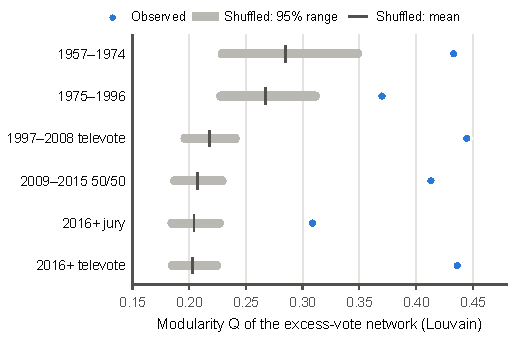
\includegraphics[width=\linewidth]{fig1_modularity}
\caption{Modularity of the excess-vote network, observed and under a shuffle null, per era. Each row is one network: one per era (1957–1974, 1975–1996, 1997–2008, 2009–2015) and, for 2016–2026, separate jury and televote networks. Nodes are countries; an edge joins two countries whose votes for each other (both directions pooled, at least 5 votes) have a positive mean excess, weighted by that mean (18–45 nodes per network). Blue dots: modularity Q of the best of five Louvain runs on the observed network. Grey bars: middle 95\% of Q over 1,000 networks in which each voter's points were randomly re-assigned among the entries it rated in the same year, round and vote type (same Louvain procedure); vertical tick: mean of the shuffled networks.}
\label{fig:fig1}
\end{figure}

\begin{figure}[tbhp]
\centering
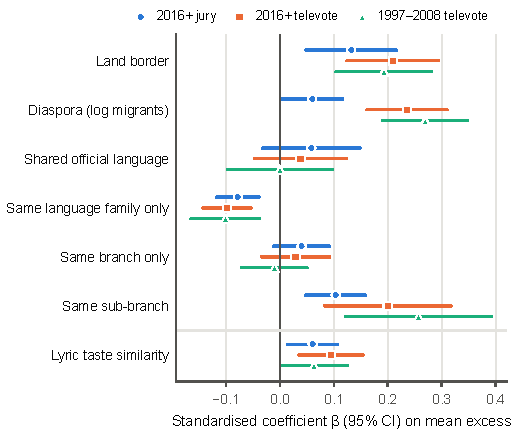
\includegraphics[width=\linewidth]{fig2_coefficients}
\caption{Standardised regression coefficients for the mean signed excess a voting country gives a receiving country. One OLS model per vote type: 2016–2026 jury (blue circles), 2016–2026 televote (orange squares) and 1997–2008 televote (green triangles); one observation per directed country pair with at least 5 votes (n = 1,537, 1,537 and 1,257 pairs). Outcome and predictors are z-scored within each model. Language family, branch and sub-branch enter as one category (deepest shared Glottolog level; reference: different families). Lyric taste similarity is the cosine similarity between the receiver's song and the voter's points-weighted lyric profile from other years, built from the same vote type. Lines: 95\% confidence intervals from standard errors clustered two-way by voting and receiving country (negative eigenvalues of the covariance set to zero, same estimator in all models). The horizontal rule separates the lyric term from the friendship terms.}
\label{fig:fig2}
\end{figure}

\begin{figure*}[tbhp]
\centering
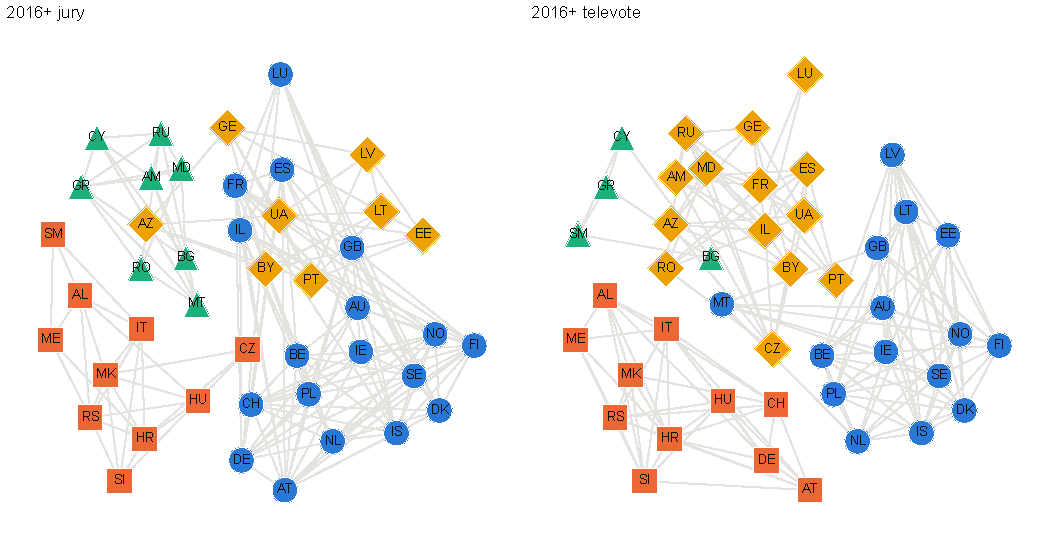
\includegraphics[width=0.9\textwidth]{fig3_communities}
\caption{Louvain communities of the 2016–2026 excess-vote networks for jury votes (left) and televotes (right), 44 countries and 4 communities in each. Marker colour and shape show community membership; a community in the televote panel gets the colour and shape of the jury community it overlaps most (one-to-one matching on the Jaccard index). Node positions are the same in both panels (one force-directed layout of the two networks combined, all edges). Grey lines: the disparity-filter backbone \cite{serrano2009backbone} of each network at $\alpha$ = 0.05, i.e. pairs (positive mean excess, both directions pooled, at least 5 votes) whose share of at least one country's positive excess is larger than a random split over its partners would give; 23 of 404 jury and 29 of 333 televote edges are kept. Solid: both countries in the same community; dashed: different communities. Labels are ISO 3166 country codes.}
\label{fig:fig3}
\end{figure*}

\begin{table*}[t]
\centering
\caption{Robustness runs. (A) Observed modularity $Q$ of the excess-vote network and its $z$-score against 1,000 shuffles, for the main edge weight (mean excess, at least 5 votes) and summed excess. (B) Standardised coefficients of the pair regression for the main model and each run that changes one choice; $^{*}$95\% CI excludes 0. Standard errors are clustered two-way by voting and receiving country with the Cameron--Gelbach--Miller eigenvalue fix; $^{\dagger}$negative eigenvalues were set to zero in that fit. The last run uses one-way clustering by voter. The last row of each block gives the range of the same-family-only coefficient when one country at a time is left out.}
\label{tab:robustness}
\small
\begin{tabular}{lcc}
\multicolumn{3}{l}{\textbf{A. Null model}} \\ \hline
Network & Mean excess, $\geq 5$ votes & Summed excess \\ \hline
1957--1974 & 0.433 (4.7) & 0.415 (4.5) \\
1975--1996 & 0.370 (4.8) & 0.346 (6.8) \\
1997--2008 televote & 0.445 (19.5) & 0.450 (25.0) \\
2009--2015 50/50 & 0.413 (19.5) & 0.411 (21.9) \\
2016+ jury & 0.309 (9.8) & 0.317 (12.6) \\
2016+ televote & 0.436 (23.3) & 0.447 (25.3) \\
2016+ televote incl. 2023--25 semis & 0.430 (22.1) & 0.448 (25.1) \\
\hline
\end{tabular}

\vspace{6pt}

\resizebox{\textwidth}{!}{%
\begin{tabular}{lrrrrrrrrr}
\multicolumn{10}{l}{\textbf{B. Regression}} \\ \hline
Run & Border & Diaspora & Shared off. lang. & Family only & Branch only & Sub-branch & Taste & $R^2$ & $n$ \\ \hline
\multicolumn{10}{l}{\textit{2016+ jury}} \\
Main model$^{\dagger}$ & $+0.13$$^{*}$ & $+0.06$$^{*}$ & $+0.06$ & $-0.08$$^{*}$ & $+0.04$ & $+0.10$$^{*}$ & $+0.06$$^{*}$ & 0.081 & 1{,}537 \\
Diaspora: listed pairs only$^{\dagger}$ & $+0.14$$^{*}$ & $+0.03$ & $+0.09$ & $-0.09$$^{*}$ & $-0.02$ & $+0.10$$^{*}$ & $+0.09$$^{*}$ & 0.103 & 1{,}015 \\
Without 5 strongest pairs$^{\dagger}$ & $+0.12$$^{*}$ & $+0.06$ & $-0.01$ & $-0.08$$^{*}$ & $+0.05$ & $+0.10$$^{*}$ & $+0.05$$^{*}$ & 0.053 & 1{,}529 \\
Taste without top-5 partners$^{\dagger}$ & $+0.13$$^{*}$ & $+0.06$$^{*}$ & $+0.06$ & $-0.08$$^{*}$ & $+0.04$ & $+0.11$$^{*}$ & $+0.04$$^{*}$ & 0.079 & 1{,}537 \\
Taste from earlier years$^{\dagger}$ & $+0.13$$^{*}$ & $+0.06$$^{*}$ & $+0.06$ & $-0.07$$^{*}$ & $+0.04$ & $+0.11$$^{*}$ & $+0.04$ & 0.079 & 1{,}537 \\
Own-song similarity$^{\dagger}$ & $+0.13$$^{*}$ & $+0.06$$^{*}$ & $+0.06$ & $-0.07$$^{*}$ & $+0.04$ & $+0.11$$^{*}$ & $+0.01$ & 0.078 & 1{,}537 \\
SEs clustered by voter only & $+0.13$$^{*}$ & $+0.06$$^{*}$ & $+0.06$ & $-0.08$$^{*}$ & $+0.04$ & $+0.10$$^{*}$ & $+0.06$$^{*}$ & 0.081 & 1{,}537 \\
\multicolumn{10}{l}{Leave one country out (43 refits): family only from $-0.087$ to $-0.066$} \\ \hline
\multicolumn{10}{l}{\textit{2016+ televote}} \\
Main model & $+0.21$$^{*}$ & $+0.24$$^{*}$ & $+0.04$ & $-0.10$$^{*}$ & $+0.03$ & $+0.20$$^{*}$ & $+0.10$$^{*}$ & 0.258 & 1{,}537 \\
Diaspora: listed pairs only & $+0.20$$^{*}$ & $+0.25$$^{*}$ & $+0.02$ & $-0.12$$^{*}$ & $+0.00$ & $+0.22$$^{*}$ & $+0.10$$^{*}$ & 0.301 & 1{,}015 \\
Without 5 strongest pairs & $+0.20$$^{*}$ & $+0.24$$^{*}$ & $+0.00$ & $-0.10$$^{*}$ & $+0.03$ & $+0.19$$^{*}$ & $+0.09$$^{*}$ & 0.227 & 1{,}529 \\
Taste without top-5 partners & $+0.22$$^{*}$ & $+0.23$$^{*}$ & $+0.04$ & $-0.10$$^{*}$ & $+0.03$ & $+0.20$$^{*}$ & $+0.05$ & 0.252 & 1{,}537 \\
Taste from earlier years & $+0.21$$^{*}$ & $+0.23$$^{*}$ & $+0.04$ & $-0.10$$^{*}$ & $+0.03$ & $+0.19$$^{*}$ & $+0.06$ & 0.253 & 1{,}537 \\
Own-song similarity & $+0.22$$^{*}$ & $+0.23$$^{*}$ & $+0.04$ & $-0.09$$^{*}$ & $+0.03$ & $+0.20$$^{*}$ & $+0.05$$^{*}$ & 0.252 & 1{,}537 \\
Incl. televote-only semis & $+0.22$$^{*}$ & $+0.23$$^{*}$ & $+0.05$ & $-0.10$$^{*}$ & $+0.03$ & $+0.20$$^{*}$ & $+0.09$$^{*}$ & 0.268 & 1{,}574 \\
SEs clustered by voter only & $+0.21$$^{*}$ & $+0.24$$^{*}$ & $+0.04$ & $-0.10$$^{*}$ & $+0.03$ & $+0.20$$^{*}$ & $+0.10$$^{*}$ & 0.258 & 1{,}537 \\
\multicolumn{10}{l}{Leave one country out (43 refits): family only from $-0.114$ to $-0.090$} \\ \hline
\multicolumn{10}{l}{\textit{1997--2008 televote}} \\
Main model & $+0.19$$^{*}$ & $+0.27$$^{*}$ & $+0.00$ & $-0.10$$^{*}$ & $-0.01$ & $+0.26$$^{*}$ & $+0.06$$^{*}$ & 0.310 & 1{,}257 \\
Diaspora: listed pairs only & $+0.18$$^{*}$ & $+0.28$$^{*}$ & $-0.01$ & $-0.10$$^{*}$ & $-0.03$ & $+0.29$$^{*}$ & $+0.06$ & 0.356 & 846 \\
Without 5 strongest pairs & $+0.18$$^{*}$ & $+0.29$$^{*}$ & $-0.03$ & $-0.11$$^{*}$ & $-0.01$ & $+0.23$$^{*}$ & $+0.07$$^{*}$ & 0.280 & 1{,}248 \\
Taste without top-5 partners & $+0.19$$^{*}$ & $+0.27$$^{*}$ & $+0.00$ & $-0.10$$^{*}$ & $-0.01$ & $+0.26$$^{*}$ & $+0.05$ & 0.308 & 1{,}257 \\
Taste from earlier years & $+0.19$$^{*}$ & $+0.27$$^{*}$ & $+0.00$ & $-0.10$$^{*}$ & $-0.01$ & $+0.25$$^{*}$ & $+0.07$$^{*}$ & 0.311 & 1{,}257 \\
Own-song similarity & $+0.19$$^{*}$ & $+0.27$$^{*}$ & $-0.00$ & $-0.09$$^{*}$ & $-0.01$ & $+0.26$$^{*}$ & $-0.00$ & 0.306 & 1{,}257 \\
SEs clustered by voter only & $+0.19$$^{*}$ & $+0.27$$^{*}$ & $+0.00$ & $-0.10$$^{*}$ & $-0.01$ & $+0.26$$^{*}$ & $+0.06$$^{*}$ & 0.310 & 1{,}257 \\
\multicolumn{10}{l}{Leave one country out (39 refits): family only from $-0.123$ to $-0.082$} \\ \hline
\end{tabular}}
\end{table*}


\section*{Discussion}
TODO (group): discussion.

% TODO (group): PNAS asks for a data / code availability statement; check where the current
% template puts it (repository URL, licences: see raw/MANIFEST.json).

\matmethods{% Generated by scripts/write_paper.py; do not edit (edit the template / figures/captions.md and rerun).
\textbf{Data.} Votes for 1957–2023 come from the Eurovision dataset of Burgoyne et al. \cite{burgoyne2023eurovision};
the 2023 semi-finals and 2024–2026 from EurovisionAPI \cite{eurovisionapi2026} (commit e564111). The table has
83,526 votes (voter, receiver, round, vote type) from 69 contests (1957–2026; 2020 cancelled);
separate jury and televote points exist from 2016. Land borders come from GeoDataSource
\cite{geodatasource_borders}; diaspora from the UN DESA International Migrant Stock 2024 \cite{undesa2024migrantstock};
official languages from Unicode CLDR 49 \cite{cldr49}; language classification from Glottolog 5.4
\cite{glottolog54}; lyrics and English translations from EurovisionAPI (1,811 of 1,830 entries have
English text). Sources, retrieval dates, checksums and licences are listed in the repository.

\textbf{Excess votes.} Each voter's points in a round were converted to shares of its points in that round.
The expected share of an entry is the mean share it received from all other voters in the same round
and vote type; excess is the observed minus the expected share. Excess removes how much everyone
liked a song that night, but not running order or staging. Eras follow the voting rules: 1957–1974,
1975–1996, 1997–2008 (televote), 2009–2015 (50/50) and 2016–2026 (jury and televote reported separately).

\textbf{Community structure.} For each era, and for 2016–2026 jury and televote separately, countries were
linked by their mean excess over all votes between them in both directions (pairs with at least
5 votes; positive weights only). Communities were found with the Louvain method
\cite{blondel2008louvain}, keeping the highest modularity $Q$ \cite{newman2006modularity} of 5 seeded runs.
In the null model each voter's set of points in a year, round and vote type was randomly re-assigned
among the entries it rated and excess recomputed (1,000 shuffles per network). We report
$z = (Q_\mathrm{obs} - \overline{Q}_\mathrm{null}) / \mathrm{SD}(Q_\mathrm{null})$.

\textbf{Pair predictors.} \textit{Border}: shared land border. \textit{Diaspora}: $\log(1 + m)$, with $m$ the number of people
born in the receiving country living in the voting country in the UN year nearest the vote; pairs the
UN does not list count as zero. \textit{Language}: shared official language (CLDR status ``official''), and the
deepest Glottolog level shared by the two countries' main languages: different families (reference),
same family only, same branch only (e.g. Slavic) or same sub-branch (e.g. South Slavic).

\textbf{Taste profile.} English lyrics were embedded with paraphrase-multilingual-mpnet-base-v2
\cite{reimers2019sentencebert}, in chunks of at most 128 tokens averaged per song, and each song vector
was centred on the mean of its year. A voter's taste profile for a vote on country $B$ in year $t$ is
the share-weighted sum of the vectors of all songs it gave points to in other years, leaving out every
song from $B$; for 2016–2026 profiles are built from jury votes and televotes separately. Taste
similarity is the cosine between the profile and $B$'s song in year $t$.

\textbf{Regression.} For each directed pair with at least 5 votes, signed excess and all predictors were
averaged over the same votes, in three samples: 2016–2026 jury and televote (1,537 pairs each)
and 1997–2008 (1,257 pairs). We fitted ordinary least squares with outcome and predictors
z-scored within each sample. Confidence intervals (95\%) use standard errors clustered two-way by voting
and receiving country \cite{cameron2011multiway}; where the two-way covariance of the reported coefficients was
not positive semi-definite (6 of 19 fits, all 2016–2026 jury), we clustered by voting country only.
All robustness runs are in Table \ref{tab:robustness}.

\textbf{Validation.} For the 2023 final the two vote sources agree on 962 of 962 votes, and the
reconstructed 2026 final matches the published scoreboard for 25 of 25 entries. Taste profiles
recomputed by a direct loop over votes agree with the vectorised computation (largest difference
$1.9\times10^{-16}$). Predictors are weakly correlated (largest $|r|$ = 0.375; largest variance inflation factor
1.39). Leaving out one country at a time, the same-family-only coefficient stays between
$-$0.123 and $-$0.066 in all three models (the 95\% CI includes 0 in 0 of 125 refits). \textbf{TODO (group):} hand ratings of 20 song pairs by two raters
(Spearman between raters and with the model), from scripts/rating\_agreement.py.
}
% What each measurement captures and misses (from RESULTS.md). Hand-written; no numbers.
\begin{table*}[t]
\centering
\caption{What each measurement captures and what it misses.}
\label{tab:measures}
\small
\begin{tabular}{p{0.16\textwidth}p{0.36\textwidth}p{0.36\textwidth}}  % widths + column gaps fit \textwidth
\hline
Measurement & Captures & Misses \\ \hline
Excess vote & how far a voter rated an entry above the other voters that night & running order, staging, performance \\
Community structure & groups giving each other more excess than reshuffled points would & why groups form; vote direction; negative excess \\
Land border & a shared land border & sea neighbours, distance \\
Diaspora & people born in the receiving country living in the voting country & later generations; migrants the census misses \\
Shared official language & an official language in common (CLDR) & mutual intelligibility; de facto and second languages \\
Language category & deepest Glottolog level the main languages share & closeness below sub-branch; minority languages \\
Taste similarity & closeness of $B$'s lyrics to lyrics the voter rewarded in other years & music, genre, staging; voter's other friendships \\
Own-song similarity & closeness of the voter's and $B$'s lyrics in the same year & what the voter actually rewards \\
NMI & overlap of two partitions (jury vs televote communities; communities vs language branch) & which groups match; rises with the number of groups \\
Attribute assortativity & positive-excess edges joining countries of the same language branch or UN sub-region & edge weights (computed unweighted); closeness between different labels; CLDR puts Cyprus in Western Asia \\
Disparity backbone & partners that get more of a country's positive excess than an even split would give & negative excess; direction; the choice of $\alpha$ \\
\hline
\end{tabular}
\end{table*}
   % what each measurement captures / misses (Table \ref{tab:measures})
\showmatmethods{}

\acknow{TODO (group): acknowledgements.}
\showacknow{}

\bibliography{references}

\end{document}
